\section{Network Layer}
\paragraph{Schicht 3: Internet}

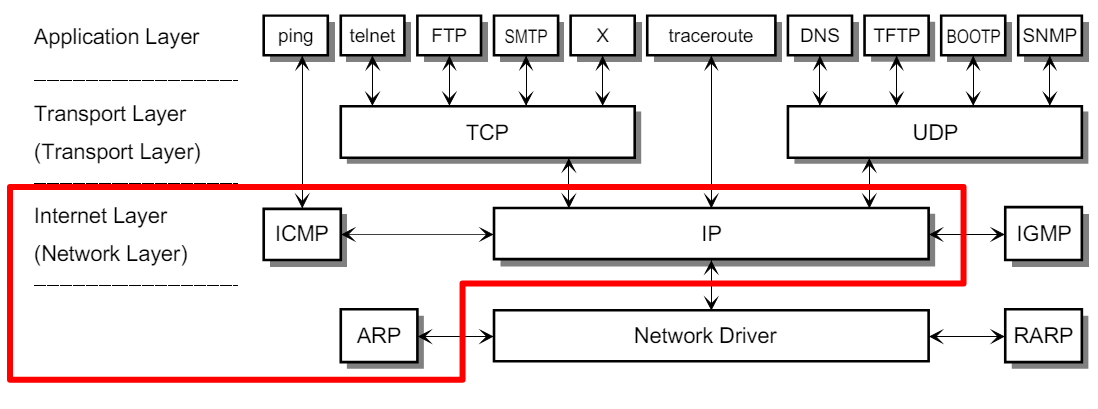
\includegraphics[width=1\linewidth]{images/orientierung_network_layer.png}

\begin{definition}{Die Netzwerkschicht}\\
    NUR Transport der IP-Pakete $\rightarrow$ höhere Layer übernehmen:
        \begin{itemize}
            \item Fehlerfreie, komplette Übertragung
            \item Richtige Reihenfolge, Flusskontrolle
        \end{itemize}
\end{definition}

\begin{lemma}{Grundsätze des Internets}
    \begin{itemize}
        \item Jedes Netzwerk soll für sich selbst funktionsfähig sein
        \item Die Kommunikation basiert auf «best effort»
        \item Die Verbindung der Netze erfolgt durch Black Boxes
        \item Keine zentrale Funktionssteuerung wird benötigt
    \end{itemize}
\end{lemma}

\begin{definition}{Kommunikationsobjekte} OSI Layern zugeordnet
       \begin{itemize}
        \item \textcolor{orange}{(Application-)Message/Stream} Layer 5-7
        \item \textcolor{green}{(Transport-)Paket, Datagram} Layer 4
        \item \textcolor{blue}{(IP-)Paket (früher Datagram)} Layer 3
        \item \textcolor{pink}{(HW-specific) Frame} Layer 1-2
    \end{itemize}
\end{definition}



\subsection{Netzwerk Applikationen und Protokolle}

\subsubsection{Routing}

\begin{definition}{Router} verbinden Subnetze (Ethernet, xDSL, WLAN, etc.)
    \begin{itemize}
        \item empfangen nur Pakete, die direkt an sie adressiert sind
        \item Weiterleitung erfolgt anhand der Network Layer Adresse
        \item Benutzen immer den optimalen Pfad.
    \end{itemize}
\end{definition}
    

\begin{concept}{Routing and Forwarding}
    \begin{itemize}
        \item Routing: Aufbau und Update der Routingtabellen in den Knoten
            \begin{itemize}
                \item Router müssen optimalen Pfad zu jedem Host kennen
                \item kleine oder Teilnetze: Statische Konfiguration
                \item grössere Netze: Dynamisch durch Routing-Protokolle: Topologie des Netzes ermitteln $\rightarrow$ ideale Pfade bestimmen
            \end{itemize}
        \item Forwarding: Weiterleiten der Daten
        \begin{itemize}
            \item Aufgrund von Routingtabellen Datenpakete weiterleiten
        \end{itemize}
    \end{itemize}
\end{concept}

\begin{definition}{Routing-Tabelle} Info wie jedes Netz/Interface erreicht werden kann
    
    \begin{itemize}
        \item Für Weiterleitungsentscheidung notwendige Informationen:
        \begin{itemize}
            \item Eintrag für jedes erreichbare Netz (Netzadresse, Netzmaske)
            \item Interfaces, über die die Netze erreicht werden können
            \item IP-Adresse des nächsten Routers, wenn Zielnetz nicht direkt erreicht werden kann
        \end{itemize}
        \item Eigenschaften:
        \begin{itemize}
            \item sortiert nach Länge der Netzmaske, von oben nach unten durchsucht
            \item erster Eintrag der passt wird verwendet, default Eintrag am Schluss passt immer
        \end{itemize}        
    \end{itemize}
\end{definition}

\subsubsection{IPv4}

\begin{KR}{IP-Header Format}
    Ein IP-Packet besteht aus einem Header (min. 20 Byte) und Nutzdaten.
    \begin{itemize}
        \item \textcolor{blue}{Version} IPv4 / IPv6
        \item \textcolor{blue}{IHL} Header Length in 4-Byte (20 Byte $\rightarrow$ IHL = 5)
        \item \textcolor{blue}{Type of Service} neu Differentiated Services (DS), Erlaubt Priorisierung, Einteilung der Daten in Verkehrsklassen
        \begin{itemize}
            \item DSCP: spez. Verhalten bzgl. Weiterleitung
            \item ECN: kann drohende Überlast markieren
        \end{itemize}
        \item \textcolor{blue}{Total Length} Länge des IP-Packets (Header + Nutzdaten)
        \item \textcolor{Goldenrod}{ID Number} Identifikation des IP-Pakets / Fragmente, erlaubt Identifikation zusammengehöriger Fragmente
        \item \textcolor{Goldenrod}{Flags} Kontroll-Flags für Fragmentierung (0/DF/MF)
        \item \textcolor{Goldenrod}{Fragment Offset} Gibt an, wo ein Fragment hingehört
        \item \textcolor{green}{Time to Live} anz. Sek, Hop-Counter, 0 $\rightarrow$ Paket wird verworfen
        \item \textcolor{green}{Protocol} Übergeordnetes Protokoll
        \item \textcolor{purple}{Header Checksum} verhindert fehlgeleitete Pakete ($\times $ Nutzdaten)
        \item \textcolor{purple}{Source Address} Wer das Paket ursprünglich abgesendet hat
        \item \textcolor{purple}{Destination Address} Wer das Paket schliesslich erhalten soll
        \item \textcolor{purple}{Options/Padding} variabel, füllt auf ein Vielfaches von 32Bits auf
    \end{itemize}
        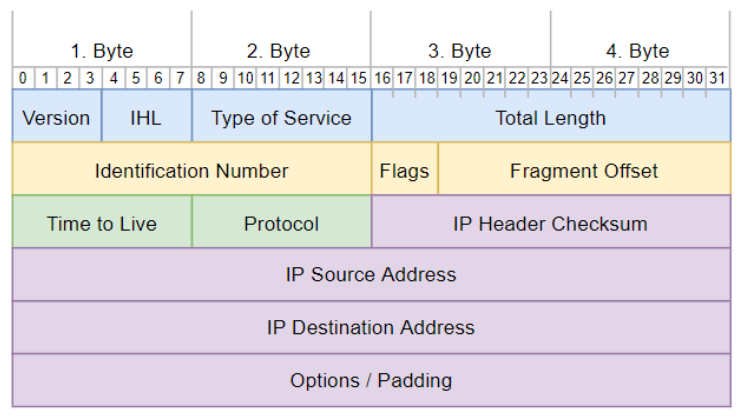
\includegraphics[width=1\linewidth]{images/internet_protokoll_format_ip.png}\\
    Das unterliegende Netz limitiert die Grösse eines Pakets (Maximum Transfer Unit). Der Sender kennt die MTU der Netze nicht.\\
\end{KR}

\begin{definition}{Fragmentierung}
    \begin{itemize}
        \item Länge der Nutzdaten = Vielfaches von 8 Bytes
        \item Die Pakete haben die gleiche und grösstmögliche Länge
        \item Identification Number, Flags und Fragment Offset (siehe \textcolor{Goldenrod}{gelbe Felder} in Grafik oben) wichtig für Fragmentierung
        \item früher von Router durchgeführt, heute im Sender
    \end{itemize}
\end{definition}

\begin{formula}{Reassembly}
    nutze Flags (0/DF/MF) und Fragment Offset
    \begin{itemize}
        \item Zusammensetzen beim Zielhost
        \item Letztes Fragment: MF = 0
    \end{itemize}
        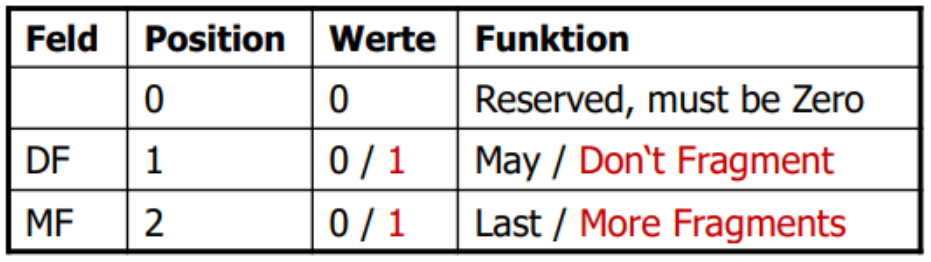
\includegraphics[width=0.75\linewidth]{images/reassembly.png}\\
        Kombination mit DF und MF erlaubt vollständige Rekonstruktion ohne explizite Übertragung der ursprünglichen Paketgrösse
\end{formula}

\subsubsection{Internet Protokolle (IP)}

\begin{definition}{Hierarchische Adressierung}\\
IP-Adressen sind zweistufig hierarchisch
\begin{itemize}
    \item IP-Adresse eines Hosts = Netzadresse + Interface-Adresse
\end{itemize}
\end{definition}

\begin{definition}{Terminologie}
    \begin{itemize}
        \item Sender und Empfänger $\rightarrow$ Hosts
        \item IP bietet einen unzuverlässigen, verbindungslosen Dienst
        \begin{itemize}
            \item IP-Adr. identifiziert Host-Interface (nicht den Host) eindeutig innerhalb des Netzwerks
            \item Jeder Host hat min. eine Adresse, Multi-Homed Hosts mehrere
        \end{itemize}
    \end{itemize}
\end{definition}

\begin{formula}{Netzadresse}
    \begin{itemize}
        \item Reserviert: Darf nicht für Interfaces verwendet werden!
        \item Tiefste Adresse im Subnetz (Interface-Adressbits alle 0)
        \item Berechnet durch: Interface-Adresse AND Subnetzmaske
    \end{itemize}
\end{formula}

\begin{formula}{Broadcast-Adresse}
    \begin{itemize}
        \item Reserviert: adressiert alle Interfaces in einem Subnetze
        \item Höchste Adresse im Subnetz (All Ones Broadcast)
        \item Berechnet durch: Interface-Adresse OR Invertierte Subnetzmaske
    \end{itemize}
\end{formula}

\begin{concept}{Subnetzmaske}\\
    bestimmt die Grenze zwischen Netz- und Interface-Adressbits:\\
        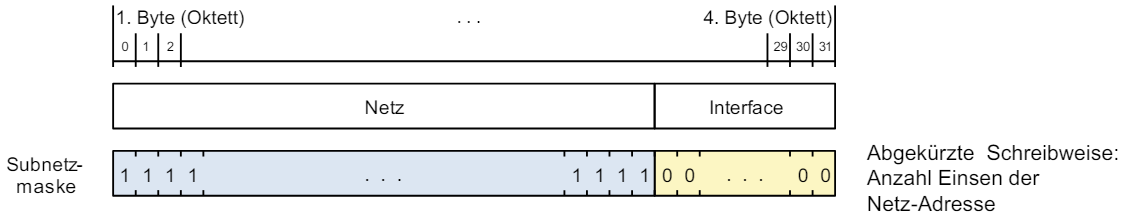
\includegraphics[width=1\linewidth]{images/subnetzmaske.png}\\
    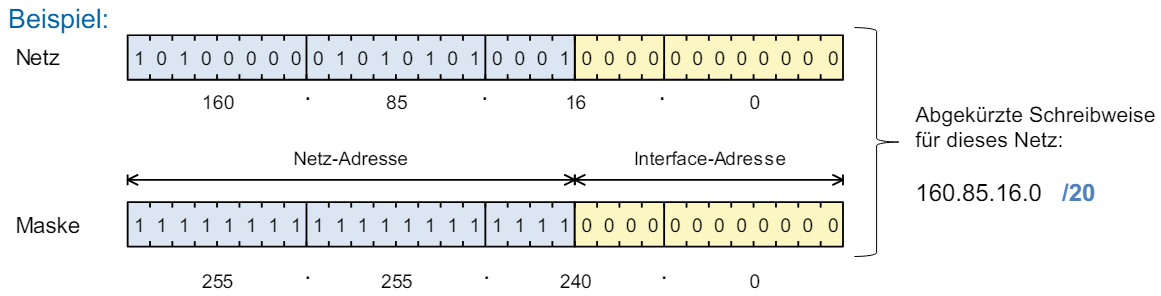
\includegraphics[width=1\linewidth]{images/subnetzmaske_bsp.png}   
\end{concept}

\begin{formula}{Netzmasken}\\
    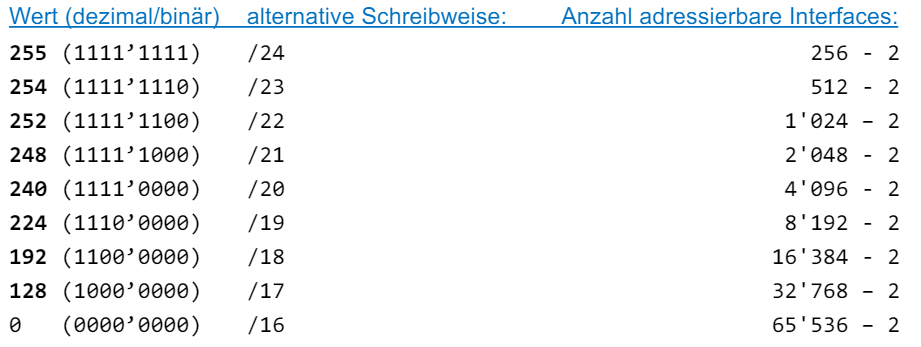
\includegraphics[width=1\linewidth]{images/subnetzmaske_bsp_2.png}
\end{formula}

\begin{KR}{Rechnen mit Netzmasken}\\
    Typische Internet-Adressen Aufgabenstellung: Berechnen Sie die fehlenden Informationen\\
        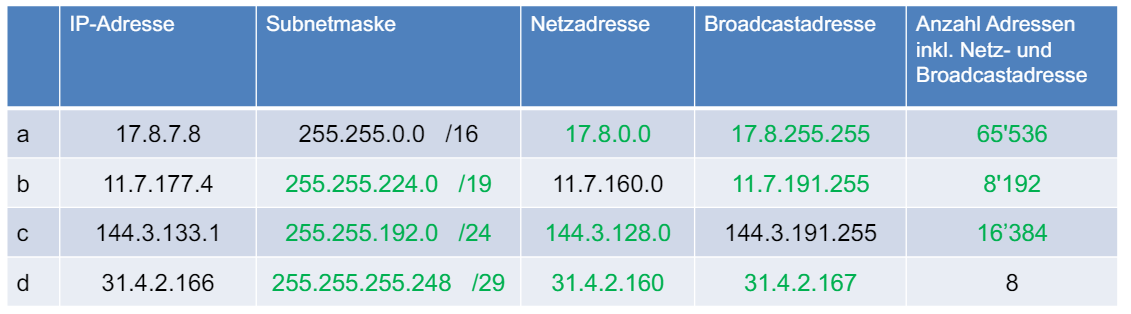
\includegraphics[width=1\linewidth]{images/rechenne_mit_netzmasken.png}
\end{KR}

\subsubsection{Flaches und Hierarchisches Routing}

\begin{concept}{Flaches Routing}
    \begin{itemize}
        \item Router kennt (evtl. mehrere) explizite Wege zu jedem Zielnetz
        \begin{itemize}
            \item Pakete an unbekannte Netze werden verworfen
        \end{itemize}
        \item Einsatz: stark vermaschte Netze oder zentraler Bereich (Backbone)
        \item Nachteil: Sehr grosse Routing-Tabellen
    \end{itemize}
\end{concept}

\begin{example2}{Flaches Routing Übung}
Was geschieht mit dem IP-Paket?
    \begin{itemize}
        \item Kein Unterbruch: Es wird nach gemäss dem 4. Eintrag der Routingtabelle von Router B an p0 weitergeleitet
        \item Unterbruch von p0/Router B: Es wird gemäss Eintrag 5 in der Routingtabelle von Router B an p2 weitergeleitet.
        \item zusätzlicher Unterbruch p0/Router C: Router C kann das IP-Paket nicht weiterleiten, es IP-Paket erreicht den Empfänger nicht.
    \end{itemize}
        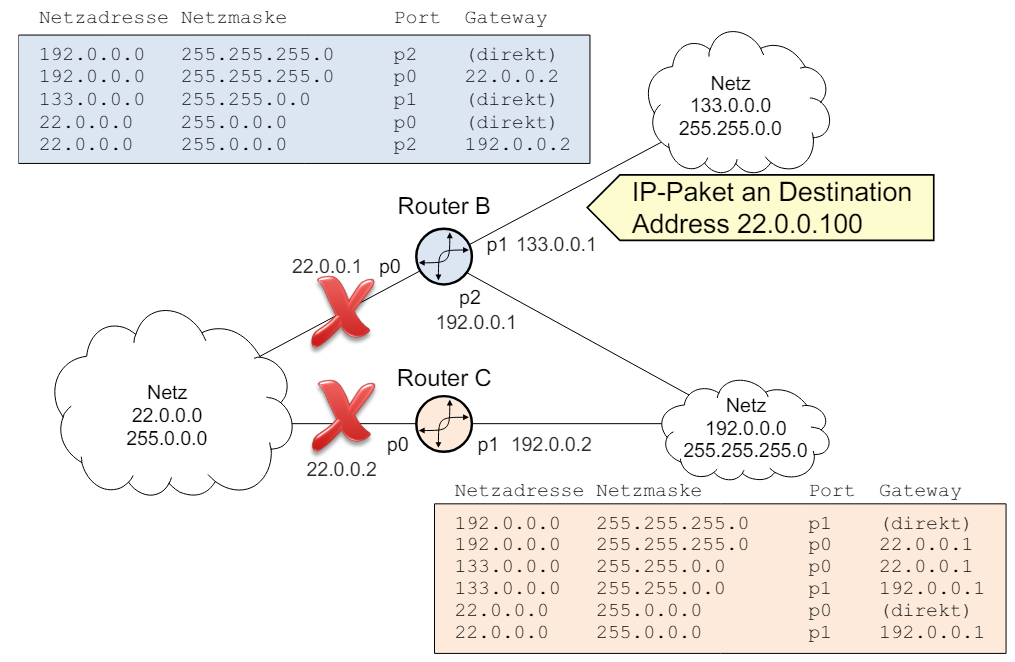
\includegraphics[width=1\linewidth]{images/flaches_routing_bsp.png}
\end{example2}

\begin{concept}{Hierarchisches Routing (Default)}
    \begin{itemize}
        \item Router kennt die direkt angeschlossenen Netze seiner Interfaces und genau einen anderen Router, an den er alles schickt, was für andere Netze bestimmt ist
        \begin{itemize}
            \item Der nächste Router geht genau gleich vor
        \end{itemize}
        \item Einsatz am „Rand“ von Netzen Hosts, ccess Router
        \item Kleine Routing-Tabellen mit jeweils einem Default-Eintrag
    \end{itemize}
        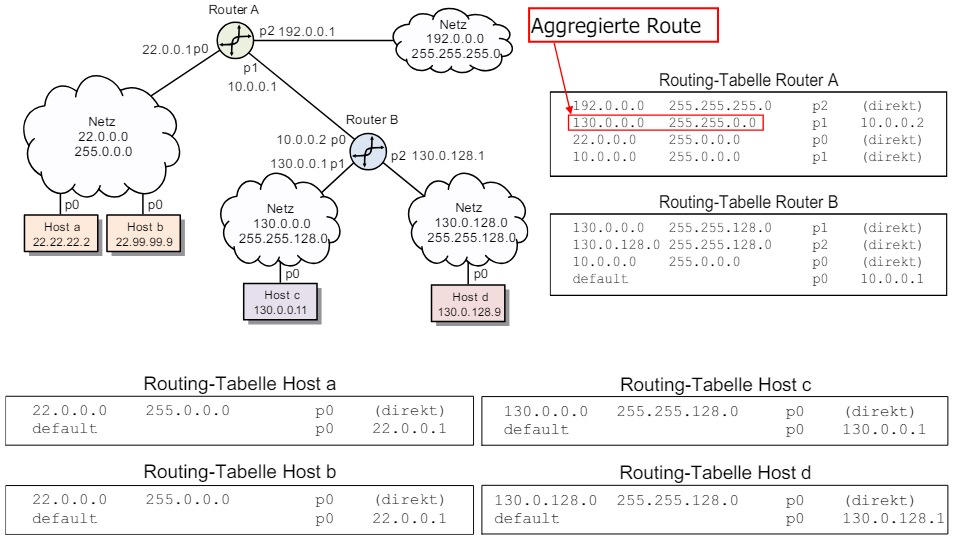
\includegraphics[width=1\linewidth]{images/hierarchisches_routing.png}
\end{concept}

\subsubsection{Classful Routing: Sub-/Supernetting}

\begin{concept}{Classful Routing}\\
    Ursprünglich war der IP Adressbereich in fünf Netzklassen (A - E) eingeteilt
    \begin{itemize}
        \item Eine Prefix (die ersten 4 Adress-Bits) erlaubt die Bestimmung der Klasse
    \end{itemize}
        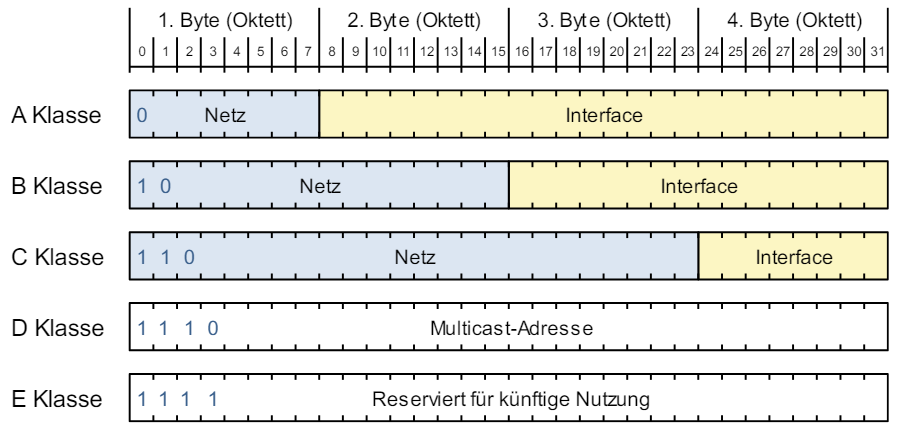
\includegraphics[width=0.9\linewidth]{images/classfulrouitng.png}
\end{concept}

\begin{KR}{Internet-Adressierung (IPv4 Netz-Klassen)}\\
    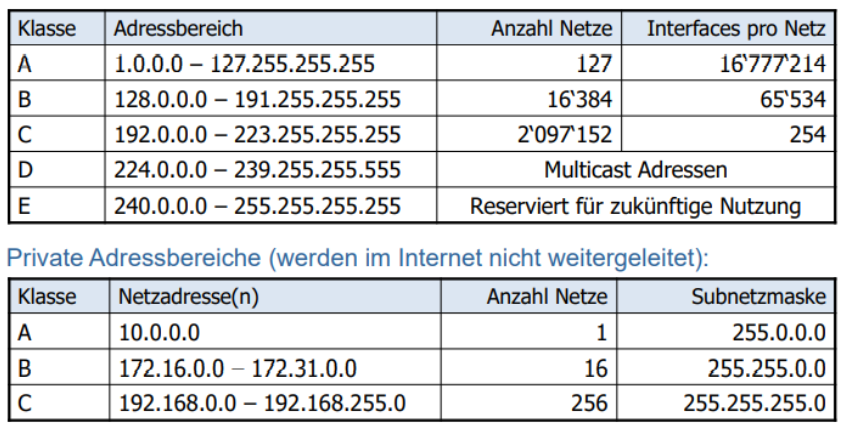
\includegraphics[width=0.8\linewidth]{images/ipv4.png}
\end{KR}

\begin{formula}{Adressbereiche für Classful Routing}
    \begin{itemize}
        \item klassische Netze fixer Grösse sind unflexibel (ungeeignet für Unternehmen)
        \\ $\rightarrow$ C zu klein, A zu gross, B zu wenig
        \item Abhilfe schafft CIDR – Classless Inter-Domain Routing
        \begin{itemize}
            \item Flexible Verwendung von Netzmasken beliebiger Länge
            \item Sub- und Supernetting
        \end{itemize}
    \end{itemize}
\end{formula}

\begin{definition}{localhost}
    Loopback-Adressen
    
    Das gesamte A-Netz 127.0.0.0/8 ist für Loopback-Test reserviert
\end{definition}



\paragraph*{Sub- und Supernetting}

\begin{concept}{Supernetting}
    Zusammenfügen von kleinen Netzen\\
    Hintereinanderliegende C Netze zu einem Netz zusammenfügen \\
    Bonus: Routingtabelle in Routern verkleinern (Aggregate Routes)
\end{concept}

\begin{example}
    Zusammenfassen von 4 Class C Netzen (22 = 2 Bits der Subnetzmaske)\\
        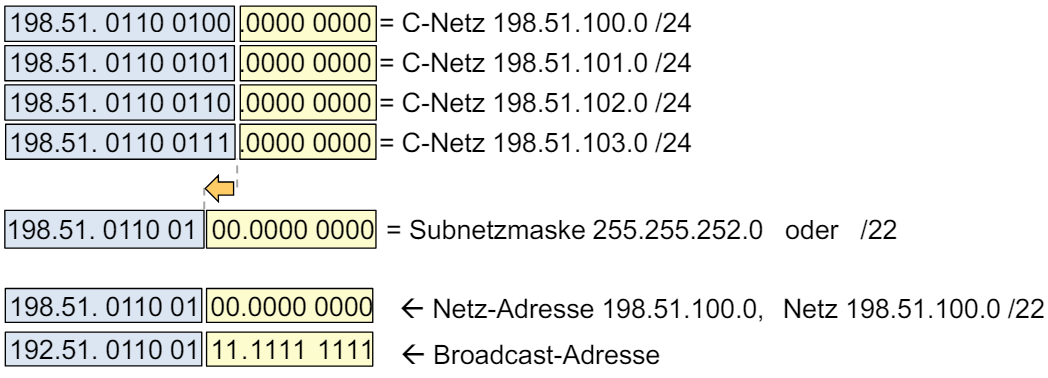
\includegraphics[width=1\linewidth]{images/example_supernetting.png}
\end{example}

\begin{concept}{Subnetting}
    Aufteilung in kleinere Netze\\
    ZHAW besitzt B Netz 160.85.0.0 $\rightarrow$ total $2^{16} \cong 65000$  Hosts
    \begin{itemize}
        \item in 8 kleinere Subnetze aufteilen $\rightarrow$ Subnetting
    \end{itemize}
    Verschieben der Netzmasken-Bits: 
    \begin{itemize}
        \item $8 = 2^3$, 3 Bits identifizieren 8 Subnetze (000 $\rightarrow$ 111) in binärer Netzmaske
        \item Netzmaske: /16 zu /19 (255.255.0.0 $\rightarrow$ 255.255.224.0)
        \item Interface-Anteil: $2^{16}$ zu $2^{13}$ = 8192 IP Adressen pro Subnetz
    \end{itemize}
        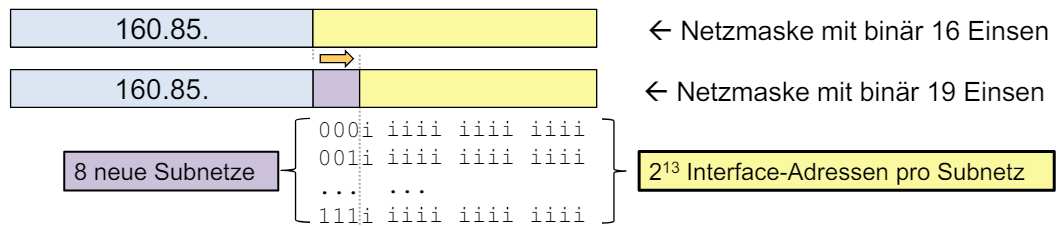
\includegraphics[width=1\linewidth]{images/subnetting1.png}\\
    Damit haben wir 8 neue Subnetze mit den folgenden Netzadressen:\\
        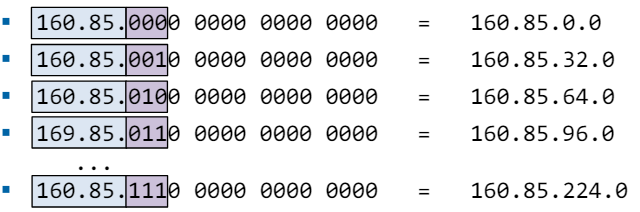
\includegraphics[width=0.75\linewidth]{images/subnetting2.png}
    \begin{itemize}
        \item Netz-Anteil: 19 statt 16 "1" $\rightarrow$ Subnetzmaske: 255.255.224.0 oder /19
        \item Host-Anteil: 13 statt 16 "0" $\rightarrow$ Anzahl Hostadressen = 8'192
    \end{itemize}
    Das zweite Netz oben wird deshalb korrekt wie folgt gekennzeichnet:
    \begin{itemize}
        \item 160.85.32.0 / 255.255.224.0 oder 160.85.32.0 /19
    \end{itemize}
    Das fünfte Netz wird wie folgt gekennzeichnet:
    \begin{itemize}
        \item 160.85.128.0 / 255.255.224.0 oder 160.85.128.0 /19
    \end{itemize}
    \textcolor{pink}{Wichtige Regel: Eine Netzwerkadresse ist immer ein Vielfaches der Netzgrösse!}
\end{concept}

\begin{example2}{Flexible Aufteilung eines Netzbereiches}\\
    4 Standorte, von ISP Netz 193.72.32.0 /21 erhalten. Ziel: 3 grössere und einen kleineren Standort redundant verbinden.\\
        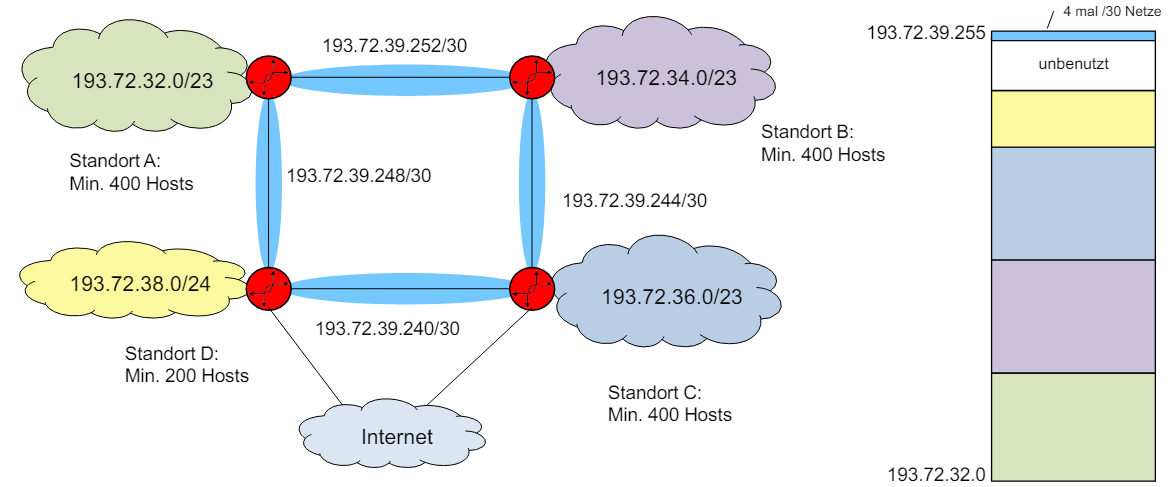
\includegraphics[width=1\linewidth]{images/flexible_aufteilung_netzbereich.png}    
\end{example2}



\subsubsection{IPv6}

\begin{definition}{IPv6} RFC 2460
    \begin{itemize}
        \item 128-bit Adressen; je zwei-Bytes in Hex-Darstellung, durch Doppelpunkte getrennt
        \item Extension Headers, um den Basic Header zu vereinfachen
        \item Interface >1 IPv6 Adressen (lokal, global, MAC-basiert, Hardware-unabhängig)
        \item verwendet zur Abfrage der Layer-2 Adressen NDP statt ARP
        \item Domain Name Service (DNS): AAAA-Records (IPv4 A-Records)
        \item Probleme: schwieriger Lesbar als IPv4, nicht rückwärtskompatibel
    \end{itemize}
\end{definition}

\columnbreak

\subsubsection{Kapselung und Adressauflösung}

\begin{definition}{Kapselung eines IP-Pakets im Ethernet Frame} von Type 0x0806\\
        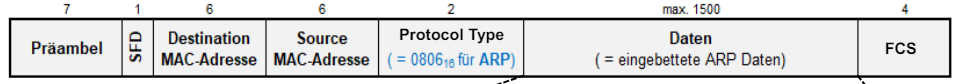
\includegraphics[width=1\linewidth]{images/kapselung_ip_paket.png}
\end{definition}



\paragraph*{Address Resolution Protocol (ARP)}

\begin{concept}{ARP}
    Ermittlung der Hardwareadresse (MAC) zu einer IP-Adresse
    \begin{itemize}
        \item ARP-Request wird an Broadcast-Adresse gesendet
        \item ARP-Response wird von Knoten mit angefragter IP-Adresse an Absender gesendet
    \end{itemize}
        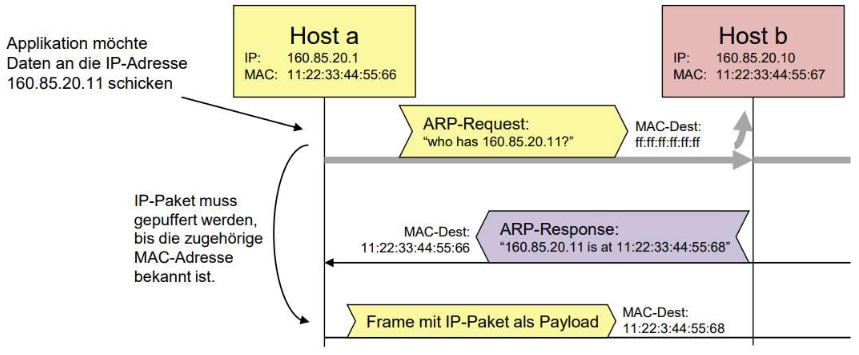
\includegraphics[width=1\linewidth]{images/arp_concept.png}
\end{concept}

\begin{remark}
    Erkennung von Adresskonflikten: ARP Request an eigene IP-Adresse
\end{remark}

\begin{formula}{ARP Nachrichtenstruktur}\\
        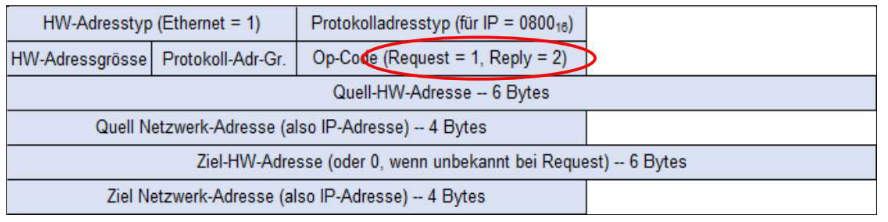
\includegraphics[width=1\linewidth]{images/arp_nachrichtenstruktur.png}
\end{formula}

\begin{remark}
    Request: Destination Address = Broadcast, HW Address of Target = 0
\end{remark}

\begin{KR}{ARP Cache} mit bekannten HW-Adressen\\
    ARP für jedes IP-Paket ineffizient $\rightarrow$ Jeder Knoten führt ARP-Cache (speichert bekannte IP-MAC Kombinationen für gewisse Zeit)
\end{KR}

\begin{example}
    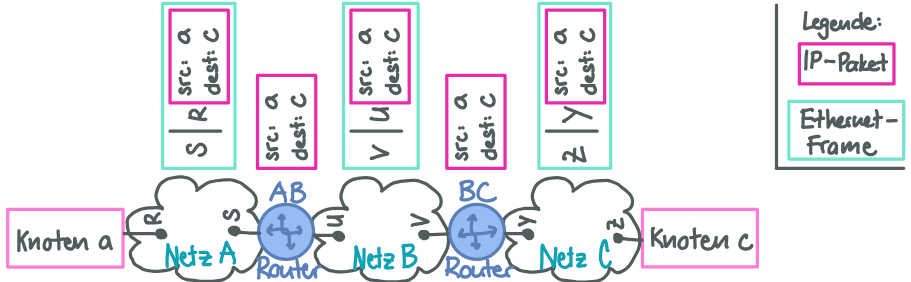
\includegraphics[width=1\linewidth]{images/encapsulation_bsp.png}\\
    \begin{itemize}
        \item a sendet IP-Paket c (Enthält Adressen a und c)
        \item a konsultiert Routing Tabelle $\rightarrow$ c kann über Router AB erreicht werden und a kennt nun IP-Adresse von Router AB
        \item a generiert Ethernet Frame, welches an HW-Adresse S von Router AB gesendet wird
        \begin{itemize}
            \item a muss aus IP-Adresse von Router AB die HW-Adresse S herausfinden $\rightarrow$ Adressauflösung
        \end{itemize}
        \item Router AB empfängt Ethernet Frame, packt IP-Paket aus und modifiziert den Header (TTL)
        \item Router AB konsultiert Routing Tabelle $\rightarrow$ c kann über Router BC erreicht werden und AB kennt nun IP-Adresse von BC
    \end{itemize}
    \textcolor{pink}{IP-Adressen a und c bleiben unverändert!}
\end{example}



\paragraph{Internet Control Message Protocol (ICMP)}

\begin{concept}{Internet Control Message Protocol (ICMP)}\\
    Übertragung von Fehlermeldungen oder Informationsaustausch
    \begin{itemize}
        \item nutzt direkt IP - keine Garantie, dass Meldungen ankommen
        \item Meldungen sind NUR informativ gedacht
    \end{itemize}
\end{concept}

\begin{KR}{ICMP Format}
    Header:
    \begin{itemize}
        \item \textcolor{blue}{Type} ICMP Typ
        \item \textcolor{green}{Code} Message Details
        \item \textcolor{green}{Checksum} Prüfsumme über die ICMP Meldung
        \item \textcolor{pink}{depends on code} Wert/Verwendung je nach ICMP Typ
    \end{itemize}
    \textcolor{purple}{Datenbereich} IP-Header und 64 Bits of Original Datagram
    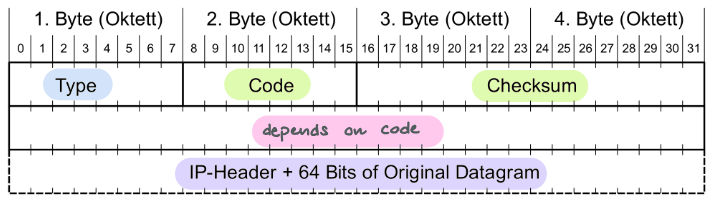
\includegraphics[width=1\linewidth]{images/icmp_details.png}
\end{KR}

\begin{formula}{ICMP Meldungstypen}

    \begin{minipage}{0.5\linewidth}
        \begin{itemize}
            \item 0: Echo Reply
            \item 3: Destination Unreachable
            \item 5: Redirect
            \item 8: Echo Request
        \end{itemize}
    \end{minipage}
    \begin{minipage}{0.5\linewidth}
        \begin{itemize}
            \item 11: Time Exceeded
            \item 12: Parameter Problem
            \item 13: Timestamp Request
            \item 14: Timestamp Reply
        \end{itemize}
    \end{minipage}
\end{formula}

\begin{definition}{ICMP Destination Unreachable}
    Router/Zielhost $\rightarrow$ Absender\\ wenn Paket nicht weitergeleitet werden kann\\
        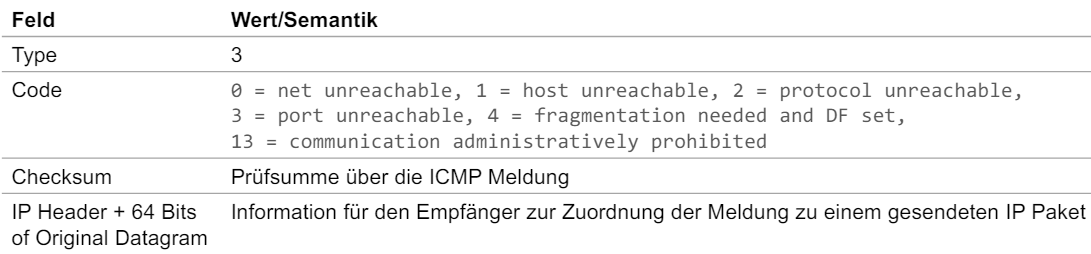
\includegraphics[width=1\linewidth]{images/destination_unreachable.png}
\end{definition}


\begin{KR}{Path MTU discovery} Vermeidung von Fragmentierung «unterwegs»\\
    Dazu: Erkennung der kleinsten MTU auf Pfad zwischen Sender und Empfänger (Path-MTU, PMTU)
    
    Vorgehen: (Annahme PMTU = lokale MTU)
    \begin{itemize}
        \item Sende IP-Pakete mit Länge=PMTU und mit DF=1
        \item Empfange «Destination Unreachable» mit Code 4 «fragmentation needed and DF set»
        \item PMTU reduzieren auf «Next-Hop MTU» (enthalten in Octet 5..8)
    \end{itemize}
\end{KR}

\begin{example2}{ICMP Destination Unreachable} Farben siehe IP-Header def.\\
    Host 160.85.31.3 sendet an Host 160.85.29.99:
    \begin{itemize}
        \item \textcolor{blue}{4500 0028} \textcolor{yellow}{8b10 0000} \textcolor{green}{0711} \textcolor{purple}{a8a4 \colorbox{lightgrey}{a055 1f03} \colorbox{lightgrey}{a055 1d63} 8b0d 829d 0014 a348 030a 0000 7504 1137 407c 0800}
        \item \colorbox{lightgrey}{Senderadr.}: a055 1f03, \colorbox{lightgrey}{Destinationadr.}: a055 1d63
    \end{itemize}
    Router kennt keinen Weg: sendet Destination Unreachable Message zurück:
    \begin{itemize}
        \item 4500 0038 8038 0000 fd\textbf{01} 5bc0 \colorbox{lightgrey}{a055 821e a055 1f03} \textcolor{blue}{03}\textcolor{green}{01 4bf7} \textcolor{pink}{0000 0000} \textcolor{purple}{4500 0028 8b10 0000 0711 a8a4 a055 1f03 a055 1d63 8b0d 829d 0014 a348}
        \item Erkennen dass dies ICMP Message ist: \textbf{Protocol}: 01
        \item ICMP Typ: \textcolor{blue}{Type}: 03
        \item 64 Bytes of Original Datagram: \textcolor{purple}{Original Data}
    \end{itemize}
\end{example2}













